Dette kapitlet beskriver produktidéens gjennomførbarhet gjennom analyse av 
dens markedsverdi. Her veies produksjonskostnad opp mot salgspris og kvantitet.
Resultatene ligger til grunne for markedstilnærmelse, salg og fortjeneste.

\section{Prisestimat}
Tabell \ref{tab:price-HW} viser en oversikt over estimert kostnad for 
hardwaren som utgjør AutoNuts-systemet, og som dermed må integreres i lastebilen. Alle estimater er ekskludert tilleggskostnader som MVA og frakt.
\newline
\begin{table}[H]
\caption{Prisestimat hardwarekomponenter i Norske kroner.}
\label{tab:price-HW}
\begin{tabularx}{\textwidth}{lcc|r}
	{\bf Del} & {\bf Antall} & {\bf Pris pr. enhet} & {\bf Subtotal}\\
	\hline
	Vibrasjonssensor (piezoelektrisk accelerometer) & 6 & 14 & 84\\
	Mikrokontroller & 3 & 10 & 30\\
	Kabler & 3 & 2 & 6\\
	\hline
	\multicolumn{3}{l}{{\bf Total (NOK)}} &\multicolumn{1}{r}{120}\\
	\hline \hline
\end{tabularx} 
\end{table}

Som vist i tabellen over, estimeres det 6 vibrasjonssensorer per lastebil. Dette
tilsvarer 2 per aksling, gitt at en lastebil har 3 akslinger. Per aksling 
estimeres også én mikrokontroller, og 1 kabel. Dette gir en 
total på 120 kr. per lastebil, og en subtotal på 40 kr. per aksling. \cite{PCBmail}

Produksjonskostnaden for teamet vil, i tillegg til innkjøpsestimatet gjort 
ovenfor, være i dagsverk. Det anslås et minimum på 720 dagsverk fra 
planlegging til produksjon. Kostnadsestimatet per dagsverk er 1200 kr. Dette gir en totalkostnad for systemutviklingen på 864000 kr.

\section{Break even}
Det økonomiske målet med prosjektet er i første omgang å nå ``break even'', 
som vil si å gå i null. Figur \ref{fig:breakeven} viser forholdet mellom 
produksjons- og innstallasjonskostnad og salgsinntekter før produktet når 
vendepunktet fra underskuddsprosjekt til profitt. 
	\newline
	\begin{figure}[H]
		\centering
		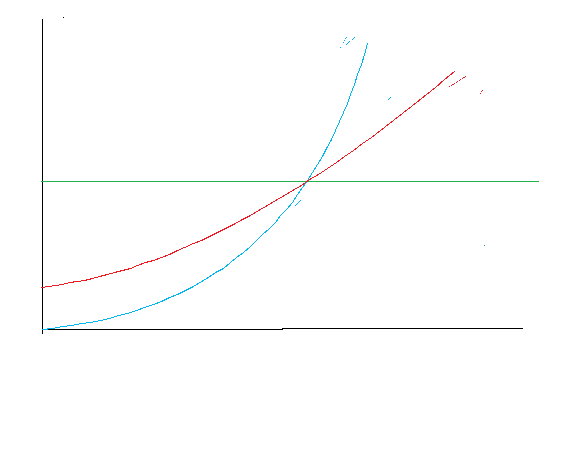
\includegraphics[width=0.80\textwidth]{images/break-even.png}
		\caption{Break even: Kostnad vs profitt.}
		\label{fig:breakeven}
	\end{figure}
X-aksen viser antall solgte ferdigmonterte enheter, mens Y-aksen viser 
Norske kroner. Rød graf er utgifter, blå graf er inntekter, mens grønn graf 
indikerer prosjektets ``break even'', altså hvor mange enheter som må selges 
før prosjektet går i overskudd.

Kongsberg Automotives representanter anbefalte en salgspris på maksimum 100 kr.
per aksling, noe som gir en total på 300 kr. per bil. Medregnet de anslåtte 
dagsverk, må det beregnes et salg på 4800 enheter før prosjektet går i overskudd.

\section{Markedsadgang}
Ettermontering av produktet vil være dyrere enn montering under produksjon av 
lastebil, man må koble fra akslingen for å montere vibrasjonssensor, samt 
trekke kabler og oppdatere software. Ettersom produktet vil bli rimeligst 
dersom det monteres under produksjon av lastebil, vil  samarbeid med en stor 
produsent, slik som feks. Volvo eller Scania være nødvendig for å entre markedet. Vi vil med andre ord være en egen bedrift som samarbeider med en lastebilprodusent for å få solgt produktet.

\section{Størrelse på marked}
Over de siste fire årene har det blitt produsert over 200 000 lasterbiler årlig 
i Europa \cite{lastebilprod-DAF}. Det vil si at markedet for produktet er 
veldig stort og vi har muligheten til å komme på markedet først. I tillegg er 
det mulighet for gjøre veien tryggere, da færre hjul vil løsne på lastebiler 
som har produktet integrert.

\section{Konkurrenter}
Til nå er det ingen konkurrenter i markedet som har en digital løsning for 
automatisk deteksjon og varsling av løse hjulbolter. Det man kan finne på 
markedet i dag er manuelle løsninger, hvor man fester små indikatorer på 
boltene for å se om de har beveget seg, eller for å feste boltene bedre, som nevnt i kapittel \ref{sec:existing-solutions}.

Vi ønsker å inngå samarbeid med store aktører for å oppnå en nisjerolle i 
markedet. På denne måten ser vi for oss å bli den foretrukne 
underleverandøren av automatisk deteksjon og varsling av løse hjulbolter.

\section{Kundens makt}
Selv om vi har fordelen med å være først ute på markedet med digital/automatisk løsning vil det være flere å konkurrere med om kundene. Dersom vi er først ut i markedet vil 
vi raskt kunne oppnå en god dialog med kundene. Vi vil etablere oss som en 
fleksibel, løsningsorientert og pålitelig leverandør. Det stilles høye krav 
til komponenter som produseres til lastebiler, siden komponentene skal være i 
drift gjennom en lang levetid. Vi vil derfor ha fokus på å levere produkter 
av høy kvalitet til en god pris. Med et stort fokus på 
kvalitetssikring sikrer vi at ingen produkter med feil havner hos 
sluttbruker. Vi ønsker fornøyde kunder og er derfor mottakelige for nye 
standarder og krav fra kundene. 

\section{Forhold til leverandører}
Det er viktig at vi velger underleverandører som er anerkjent for å levere 
komponenter med høy kvalitet og pålitelighet. Samtidig må vi forholde oss til 
pris på komponenter fra underleverandører, da det vil være vanskelig å få 
solgt produktet til kunder om prisen er for høy. Vi skal kjøpe 
prøveeksemplarer fra forskjellige leverandører for å kunne sammenligne pris 
mot kvalitet. Vi skal sikre gode avtaler med underleverandørene, og binder en 
mindre del av vår kapital på lagerhold om vi har underleverandører som 
leverer komponenter på kort varsel. Vi forhandler frem langsiktige kontrakter 
for å sikre leveranse og pris, med forbehold om brudd ved mislighold av krav 
på kvalitet, pris og levering. 

\section{De fire P-ene}
\begin{description}
	\item[Produktstrategi] Etter lansering av produktet skal vi jobbe med videreutvikling av produktet, så lenge det er mulig å skape verdi. Det vil da være aktuelt å se på andre problemer som kan detekteres ved bruk av 			samme sensor. Med tid vil vi da kunne tilby et større produkt, og kunden vil kunne få mer 			funksjonalitet for pengene. Denne videreutviklingen vil fortsette etter de tre årene, helt til all aktuell 		funksjonalitet er implementert.
	\item[Prisstrategi] Delene som kreves for å lage produktet koster ca. 40 kr per aksling for å gjør integrering av produktet mulig. Ettersom vi ikke har innsikt i den eventuelle samarbeidspartnerens økonomi, vil prising av produktet være opp til salgsavdelingen deres. Vi ser for oss en fordeling av inntekter hvor vi får 40\%, mens samarbeidspartner får 60\%. Etter hvert som bedriften skaffer seg egenkapital vil det være naturlig å gjøre enda større avtaler med underleverandører og samarbeidspartnerer. Dette vil resultere i lavere kostnader ved innkjøp av komponenter og høyere fortjeneste ved salg.
	\item[Distribusjon og salgsstrategi] Vi planlegger å selge produktet til produsenter av lastebiler. De 		skal selge produktet til sine kunder som et tilleggsprodukt eller innbakt i prisen på lastebilen. 			Distribusjon vil derfor gå gjennom produsenter, og fokuset vårt vil være å inngå avtaler med 			produsenter. Vi ser for oss å starte med salg i Europa først, hvor de vil være naturlig å inngå samarbeid med store europeiske produsenter slik som Volvo, Mercedez og Scania. Når salget i Europa har stabilisert seg ønsker vi å gå videre med salg og distribusjon globalt.  Da ser vi for oss samarbeid med store produsenter, slik som Daimler \cite{daimler}. Daimler er verdens største globale produsent av 				trailere over 6 tonn og produsererfor merkene Mercedez, Freightliner, Western Star, Fuso og 			BharatBenz \cite{daimler}.
	\item[Promoteringsstrategi] Vi planlegger å ha stand på konferanser og messer hvor vi vil vise hvordan vårt 	produkt kan automatisk detetektere og varsle om løse hjulbolter. Her vil vi få kontakt med 			lastebilprodusenter og vise at vårt produkt vil tjene deres produkt. Promotering av produktet vil 		inngå i kundens promotering ut til sluttbruker, da produktet vil være en del av kundens produkt. 		Både kunder og 	sluttbruker vil ha tilgang til informasjon om våre produkter gjennom vår nettside.
\end{description}
